% Informal research notes for collaborators, 2026-11-18. Numbers trace to REPORT.md and STATUS.md of the cd-conjecture
% repository. Figures: make_figs.py in this folder.
\documentclass[11pt]{article}
\usepackage[margin=1in]{geometry}
\usepackage{amsmath,amssymb}
\usepackage{graphicx}
\usepackage{booktabs}
\usepackage[compact]{titlesec}
\usepackage{titling}
\usepackage{enumitem}
\usepackage{multicol}
\usepackage[colorlinks=true,linkcolor=blue,citecolor=blue,urlcolor=blue]{hyperref}
\setlength{\droptitle}{-9ex}
\setlength{\textfloatsep}{12pt plus 2pt minus 4pt}
\setlength{\floatsep}{10pt plus 2pt minus 2pt}
\AtBeginDocument{\setlength{\abovedisplayskip}{7pt plus 2pt minus 3pt}\setlength{\belowdisplayskip}{7pt plus 2pt minus 3pt}\setlength{\abovedisplayshortskip}{3pt plus 2pt}\setlength{\belowdisplayshortskip}{5pt plus 2pt minus 2pt}}
\pretitle{\begin{center}\Large}\posttitle{\par\end{center}\vspace{-2.5ex}}
\preauthor{}\postauthor{}
\predate{\begin{center}\small}\postdate{\par\end{center}\vspace{-3ex}}

\title{A qubit chain with $c=2$: notes}
\author{}
\date{18 November 2026}

\begin{document}
\maketitle

% ============================================================================================
\section{The question}

For a chain that flows to a $(1+1)$-dimensional conformal field theory, the entanglement entropy of a block of $\ell$ sites at the end of an open chain grows as $(c/6)\ln\ell$~\cite{HLW,VLRK,CC}, so the central charge can be read from ground states. Latorre and Sierra~\cite{LS} conjectured that if the low-energy spectrum of a translation-invariant nearest-neighbour chain on $(\mathbb C^d)^{\otimes L}$ is described by unitary conformal field theories with central charges $c_a$, then
\begin{equation}
\sum_a c_a\le d-1 .
\label{eq:cd}
\end{equation}
The bound is saturated by the $SU(d)_1$ point of the Uimin--Lai--Sutherland chains~\cite{Sutherland} and holds in every solvable example, including the Hubbard chain, where $d=4$ and the spin and charge modes give $c=2$ with different velocities~\cite{Hubbard}. For qubits it says $c\le1$.

The natural route to a second gapless boson is a second Fermi sea. A flipped spin is a hard-core particle, and a nearest-neighbour hop gives it a $\cos k$ band with one minimum; a second minimum needs a hop by two sites. The idea is to generate that hop. A strong $ZZ$ coupling forbids particles on neighbouring sites, a blockade as in Rydberg chains~\cite{FSS,Bernien}, and a pairing term $\sigma^+\sigma^+$ then moves a particle by two sites through a virtual state. With the direct hop tuned down to the same size, the band has two valleys, and a gas that fills both is a two-component Luttinger liquid with $c=2$. The mechanism is perturbative. The evidence for $c=2$ is numerical, and not all of it is converged.

% ============================================================================================
\section{The chain}

We study the chain of Pauli matrices
\begin{equation}
H=\sum_j\Big[J_xX_jX_{j+1}+J_yY_jY_{j+1}+D\,(X_jY_{j+1}-Y_jX_{j+1})+J_zZ_jZ_{j+1}+h_zZ_j\Big],
\label{eq:H}
\end{equation}
with the reference point
\begin{equation}
J_x=-J_y=\tfrac12,\qquad D=\tfrac1{160},\qquad J_z=10,\qquad h_z=-19.976047251 .
\label{eq:ref}
\end{equation}
Taking the all-up state, which the field favours, as the vacuum and a down spin as a particle, $b_j=\sigma^+_j$ with $\sigma^\pm=(X\pm iY)/2$, the in-plane part of a bond is a direct hop and a pair term,
\begin{equation}
\begin{gathered}
J_xXX+J_yYY+D\,(XY-YX)=t_1\,b^\dagger_{j+1}b_j+\Delta\,b_jb_{j+1}+\mathrm{h.c.},\\
t_1=J_x+J_y+2iD,\qquad \Delta=J_x-J_y .
\end{gathered}
\label{eq:particles}
\end{equation}
Neighbouring particles cost the blockade energy $V=4J_z$, and an isolated particle costs $-4J_z-2h_z$, close to zero when $h_z\approx-2J_z$: at low energy we have a gas of particles that cannot be neighbours.

The pair term always breaks the blockade, so it acts only virtually. Next to a particle at site $j$ it creates a pair on $(j+1,j+2)$, at energy $2V$, and the pair term on $(j,j+1)$ then removes the original particle together with its new neighbour. The net effect is a hop by two sites, with amplitude
\begin{equation}
t_2=-\frac{\Delta^2}{2V}.
\label{eq:t2}
\end{equation}
The direct hop is first order and must be tuned down to compete. On the line $J_x+J_y=0$ it is $t_1=2iD$, and setting $|t_1|=|t_2|$ fixes all couplings in terms of one small parameter $\varepsilon=\Delta/V$, equal to $1/40$ here:
\begin{equation}
D=\frac{\varepsilon\Delta}{4}=\frac{\Delta^2}{16J_z},\qquad J_z=\frac{\Delta}{4\varepsilon},\qquad h_z=-2J_z+O(\varepsilon\Delta).
\label{eq:eps}
\end{equation}
The remainder in the field, of order $t_2$, sets the density. At the reference point $|t_1|=|t_2|=1/80$, and as $\varepsilon\to0$ only the complex ratio $t_1/t_2$ and the density matter.

% ============================================================================================
\section{Blockaded particles with two valleys}

The second-order processes inside the blockaded space give
\begin{equation}
\begin{gathered}
H_{\rm eff}=\mathcal P\sum_j\Big[t_1\,b^\dagger_{j+1}b_j+t_2\,b^\dagger_{j+2}b_j+\mathrm{h.c.}+V_2\,n_jn_{j+2}+V_3\,n_jn_{j+3}-\mu\,n_j\Big]\mathcal P,\\
V_2=2t_2,\qquad V_3=\tfrac23t_2,
\end{gathered}
\label{eq:Heff}
\end{equation}
where $\mathcal P$ removes neighbouring occupations and $n_j=b^\dagger_jb_j$. The attractions arise because two particles two or three sites apart suppress fewer of the vacuum's virtual pairs together than apart. Number-changing terms first appear at third order. Equation~\eqref{eq:Heff} reproduces the low-lying spectrum of the 12-site qubit chain, with deviations that fall rapidly as $V/\Delta$ goes from 20 to 80. The hop by two sites passes over a site that the blockade keeps empty, so it carries no string sign, and we treat the particles as hard-core bosons. With $t_1=|t_1|e^{i\varphi}$ and $b_k=L^{-1/2}\sum_je^{ikj}b_j$, the band is
\begin{equation}
\epsilon(k)=2|t_1|\cos(k+\varphi)-2|t_2|\cos2k .
\label{eq:band}
\end{equation}
The hop by two sites alone has degenerate minima at $k=0$ and $\pi$; at $\varphi=\pi/2$ the direct hop moves them without splitting them, to
\begin{equation}
k=k_0\quad\text{and}\quad k=\pi-k_0,\qquad \sin k_0=\frac{|t_1|}{4|t_2|},
\label{eq:k0}
\end{equation}
as long as $|t_1|<4|t_2|$ (Fig.~\ref{fig:band}). The choice $|t_1|=|t_2|$ sits between losing the second valley, at $|t_1|\ge4|t_2|$, and nearly decoupled sublattices, each a ferromagnetic Heisenberg chain, as $|t_1|\to0$. Off the line the valleys are split by an energy proportional to $\pi/2-\varphi$, which acts as a field on the valley label. Besides the reference point we study $t_1=e^{1.53i}/80$, which adds a small $XX+YY$ term. There the splitting is $0.16|t_2|$, and the valleys are filled in a ratio of about $57{:}43$ (effective model at density $3/16$).

\begin{figure}[t]
\begin{minipage}[c]{0.47\textwidth}
\centering
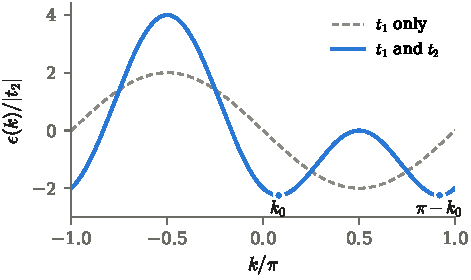
\includegraphics[width=\textwidth]{notes_qubit_fig1.pdf}
\end{minipage}\hfill
\begin{minipage}[c]{0.49\textwidth}
\centering\small
\begin{tabular}{lll}
\toprule
 & reference & $\varphi=1.53$\\
\midrule
$J_x$ & $1/2$ & $0.5002549$\\
$J_y$ & $-1/2$ & $-0.4997451$\\
$D$ & $1/160$ & $0.0062448$\\
$J_z$ & $10$ & $10$\\
$h_z$ & $-19.976047251$ & $-19.97589125$\\
$n$ & $0.19$ & $0.215$\\
\bottomrule
\end{tabular}
\end{minipage}
\caption{\label{fig:band}Left: the band~\eqref{eq:band} at $\varphi=\pi/2$ and $|t_1|=|t_2|$ (solid), with minima at $k_0=\arcsin\frac14$ and $\pi-k_0$, and the direct hop alone (dashed). Right: the two points studied, both with $\Delta=1$, $V=40$, $|t_1|=|t_2|=1/80$; $n$ is the mid-chain density at $L=256$ and 512.}
\end{figure}

A gas filling both valleys has one boson per valley, with phase $\theta_{a,b}$ and density field $\phi_{a,b}$. With $\theta_{c,s}=(\theta_a\pm\theta_b)/\sqrt2$, likewise for $\phi$, and the conventions of Ref.~\cite{Giamarchi},
\begin{equation}
H=\sum_{\nu=c,s}\frac{v_\nu}{2\pi}\int dx\,\Big[K_\nu(\partial_x\theta_\nu)^2+\frac1{K_\nu}(\partial_x\phi_\nu)^2\Big]+g_s\int dx\,\cos\big(\sqrt8\,\phi_s\big),
\label{eq:LL}
\end{equation}
where $e^{im\theta_\nu}$ has scaling dimension $m^2/4K_\nu$ and $e^{im\phi_\nu}$ has $m^2K_\nu/4$. The quadratic part is two $c=1$ theories with unrelated velocities. On the line $\varphi=\pi/2$, with particle number conserved and the density incommensurate, the only zero-momentum operator that can gap a mode is the inter-valley backscattering $g_s$, of dimension $2K_s$. The Luttinger parameters follow from two exponents,
\begin{equation}
\langle b^\dagger_jb_{j+r}\rangle\sim r^{-\eta_b},\quad \eta_b=\frac1{4K_c}+\frac1{4K_s};\qquad
\langle P^\dagger_jP_{j+r}\rangle\sim r^{-\eta_{\rm pair}},\quad \eta_{\rm pair}=\frac1{K_c},
\label{eq:exponents}
\end{equation}
up to oscillating factors, with $P$ the inter-valley pair, of momentum near $\pi$ (the valley fields are mutually bosonic, which we checked on two-body spectra).

% ============================================================================================
\section{The danger: inter-valley pairing}

If $K_s<1$, the backscattering locks $\phi_s$ and gaps the pseudospin mode, leaving a liquid of inter-valley pairs with $c=1$. In the dilute limit this happens. Two particles from different valleys feel the hard core at separations $0,\pm1$ and the attractions at $\pm2,\pm3$, and at $|t_1|=|t_2|$, $\varphi=\pi/2$ they bind, into a pair of total momentum $k_0+(\pi-k_0)=\pi$, about 21 sites across, with binding energy $E_b\approx0.020|t_2|$ (from the scattering problem and from exact diagonalization on large rings). Without $V_2$ and $V_3$ they do not bind.

The pair is large and shallow, and it can come apart at finite density. Feeding the two-body scattering data into the low-energy theory, before measuring $K_s$, we predicted $K_s\approx1.3$ to $1.7$ (each $\pm0.2$) at $n=1/8$ to $3/16$, with $K_s=1$ at $n_c\approx0.07$ to $0.085$: a pair liquid with $c=1$ below $n_c$, and a two-component liquid with $c=2$ above. Both points studied lie above $n_c$ by more than a factor of two.

% ============================================================================================
\section{Evidence}

\subsection{The effective model}

We solved Eq.~\eqref{eq:Heff} on the infinite chain with infinite DMRG~\cite{McCulloch}, with the blockade and particle number exact. At bond dimension $\chi$ a critical state has a finite correlation length $\xi$, and~\cite{CC,Tagliacozzo,Pollmann}
\begin{equation}
S=\frac c6\ln\xi+\text{const}.
\label{eq:fes}
\end{equation}
We fit $c$ over the four largest $\chi$ and follow the pseudospin and charge correlation lengths separately; a pseudospin gap shows up as a pseudospin length that stops growing while the charge length keeps growing. At $n=3/16$, $1/8$ and $1/6$ the chain reads $c=1.996$, $1.995$ and $1.993$, out to $\xi=645$, $748$ and $532$ sites, and the ratio of the two lengths is stable to one percent over the last doubling of $\chi$. An exact $c=2$ gas in the same band reads $1.988$ at $\xi=680$, and hard rods ($c=1$) read $0.987$.

To check that the method sees a gap where there is one, we followed it down in density (Fig.~\ref{fig:gap}). On open chains up to 256 sites (288 at $n=1/48$) the pair-breaking gap
\begin{equation}
\Delta_{\rm pb}=E(N+1)+E(N-1)-2E(N)
\label{eq:pb}
\end{equation}
extrapolates to $0.013|t_2|$ at $n=1/48$, falling to $0.0012|t_2|$ at $n=1/16$ (errors $0.001$ to $0.003$), and to zero within errors at $n=1/8$, $5/32$ and $3/16$. On the infinite chain, over the last doubling of $\chi$, the pseudospin length grows by only $1.06$ and $1.14$ at $n=1/32$ and $1/24$ while the charge length doubles, and $c=1.01$ and $1.04$: a pair liquid. From $n=3/40$ up both lengths grow together and $c=1.97$ to $2.00$. The gap closes between $n=1/16$ and $3/40$, and fits place $n_c$ between about $0.04$ and $0.10$, as predicted.

\begin{figure}[t]
\centering
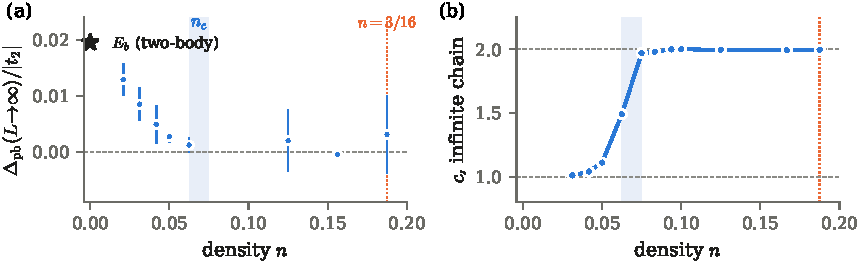
\includegraphics[width=\textwidth]{notes_qubit_fig2.pdf}
\caption{\label{fig:gap}The pair gap in the effective model at $|t_1|=|t_2|$, $\varphi=\pi/2$. (a) Pair-breaking gap extrapolated to infinite length; the star is $E_b$. (b) $c$ on the infinite chain, Eq.~\eqref{eq:fes}. Shaded: where the pseudospin length stops saturating; dotted: $n=3/16$.}
\end{figure}

At $L=256$, with fit ranges fixed on two decoupled XX chains (which give $0.502$ and $1.00$ against the exact $1/2$ and $1$), the exponents at $n=1/8$ to $3/16$ are $\eta_b=0.33$ to $0.35$ and $\eta_{\rm pair}=0.61$ to $0.64$. So $K_c\approx1.6$ ($1.8$ from the density structure factor), and $K_s=1.2$ to $1.5$: the backscattering, of dimension $2.3$ to $3.0$, is irrelevant. On small rings at $n=1/5$, exact diagonalization resolves two linear modes, with velocities $v_1\approx0.9|t_2|$ and $v_2\approx2.05|t_2|$ (the slower is most likely the pseudospin mode), and the Casimir term of the ground-state energy gives $c_1v_1+c_2v_2=2.83$ against $v_1+v_2=2.96$. As in the Hubbard chain, Eq.~\eqref{eq:cd} counts these two modes as $c=2$.

\subsection{The qubit chain}

We ran DMRG~\cite{White,Schollwock} on Eq.~\eqref{eq:H} itself, with no projection, on open chains of $L=64$ to $512$ sites, with exact parity labels, both parity sectors at every size, keeping the lower. CPU and GPU runs of the same solver agree to $3\times10^{-10}$ in energy and $10^{-6}$ in entropy. We fixed the convergence criteria and the rule for reading $c$ before the production runs. On an open chain the entropy of the first $\ell$ sites is~\cite{CC}
\begin{equation}
S(\ell)=\frac c6\ln\Big[\frac{2L}{\pi}\sin\frac{\pi\ell}{L}\Big]+s_0+\text{oscillating terms}.
\label{eq:cc}
\end{equation}
Averaging $S$ over the $2W+1$ central cuts suppresses the oscillations, and two sizes give
\begin{equation}
c(L\to2L)=\frac{6\,\big[\bar S_W(2L)-\bar S_W(L)\big]}{\ln2}.
\label{eq:ctwo}
\end{equation}
We quote $W=6$; at the two larger size pairs $W=1$ and $12$ shift the readings by at most $0.035$. We calibrate on exactly solvable chains at the same sizes (an XX chain, with hard rods in its place at the largest pair, $c=1$, and two XX chains on alternating sites, $c=2$) and on the effective model at $n=3/16$. Over $64\to128$, $128\to256$ and $256\to512$ the $c=1$ chain reads $0.94$, $0.97$, $0.99$, the $c=2$ chain $1.92$, $1.90$, $1.95$, and the effective model $1.82$, $1.88$, $1.93$. The qubit chain, at its largest bond dimension at each size ($\chi=512$, $1536$, $2048$ at $L=128$, $256$, $512$), reads about $2.2$, then $2.03$ at both points, then $1.98$ at the reference point and $1.95$ at $\varphi=1.53$ (Fig.~\ref{fig:qubit}).

\begin{figure}[t]
\centering
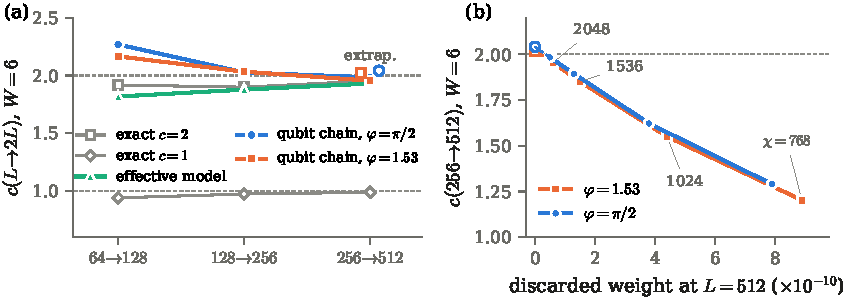
\includegraphics[width=\textwidth]{notes_qubit_fig3.pdf}
\caption{\label{fig:qubit}The qubit chain. (a) Two-size readings~\eqref{eq:ctwo} at $W=6$, each size at its largest bond dimension, with the effective model and the exact chains read the same way; open symbols are $256\to512$ extrapolated linearly in the discarded weight. (b) $c(256\to512)$ against the discarded weight at $L=512$ ($\chi=768$ to $2048$, with $L=256$ at $\chi=1536$), and the linear extrapolation.}
\end{figure}

The exact $c=2$ chain reads below 2 because of the open-boundary corrections of a two-valley Fermi sea. The effective model approaches 2 from below and the qubit chain from above, and at the largest sizes all three sit between $1.93$ and $1.98$. Before the converged $L=512$ results we fixed how to read them: $1.93$ or more would favour $c=2$ with an irrelevant correction, $1.85$ or less a slow flow toward the pair liquid. The measured $1.95$ and $1.98$ favour $c=2$, and fits of the whole profile~\eqref{eq:cc} at $L=512$ give $1.99$ and $2.00$.

Up to $L=256$ the readings are converged: the entropy moves by $0.003$ to $0.004$ between $\chi=1024$ and $1536$. At $L=512$ it rises by $0.04$, $0.031$ to $0.035$, and $0.010$ to $0.012$ over $\chi=768\to1024\to1536\to2048$ [Fig.~\ref{fig:qubit}(b)], the last step just above our tolerance of $0.01$. Because the entropy only rises with $\chi$, the $256\to512$ readings are lower bounds. Linear extrapolation in the discarded weight, which underestimates when the entropy is concave in it, as here, gives $2.01$ to $2.05$.

The Luttinger parameters match the effective model. At $L=256$ the pair exponent is $0.634$ to $0.643$ (effective model $0.623$), and $K_c$ from the structure factor is $1.70$ to $1.73$ ($1.79$ to $1.81$). $K_s$ reads $1.4$ to $1.6$ from the boson exponent and $1.84$ to $2.05$ with $K_c$ from the pair exponent, the spread coming from the open ends; every estimate is above 1.

At $\chi=768$, not yet converged, four further points nearby read $1.94$ to $2.03$ from $128$ to $256$. The reference point reads $1.94$ at $V/\Delta=80$ and $1.95$ at $V/\Delta=40$: corrections to Eq.~\eqref{eq:Heff} four times smaller leave it unchanged.

% ============================================================================================
\section{Particle number is only emergent}

The qubit chain conserves only $\prod_jZ_j$, so the $U(1)$ of the liquid is emergent. The infinite-chain results for Eq.~\eqref{eq:Heff} cannot see number-changing terms; the open qubit chains contain them but stop at 512 sites. Operators that change $N$ by two carry a pair momentum, near $\pi$ or near $\pm2k_0\approx\pm0.5$, of the order of the Fermi momenta or larger, and are not resonant. Among parity-even operators of dimension below two, only the product of two inter-valley pairs has small momentum:
\begin{equation}
\mathcal O_4=P^2+\mathrm{h.c.}\sim\cos\big(2\sqrt2\,\theta_c-q_4x\big),\qquad
\Delta_4=\frac2{K_c}=2\eta_{\rm pair},\qquad q_4=2(Q-\pi),
\label{eq:O4}
\end{equation}
with $Q$ the pair momentum; it changes $N$ by four. The measured pair exponents give $\Delta_4\approx1.25$ (effective model, on and off the line; $1.27$ to $1.29$ on the qubit chain), so $\mathcal O_4$ is relevant when resonant, with RG eigenvalue about $0.75$. On the line $Q=\pi$ and $q_4=0$; at $\varphi=1.53$ the measured pair momentum gives $q_4\approx0.015$.

The bare coupling is fourth order in the pairing: $\mathcal O_4$ is generated at second order in the third-order term, of amplitude $2\Delta^3/3V^2$, that creates two particles three sites apart, and no symmetry forbids it on the line. Relative to $|t_2|$, and with the locking length at which a resonant relevant coupling reaches order one,
\begin{equation}
g_4\approx\frac{16}{9}\,C_4\,\varepsilon^2,\qquad \xi_4\sim a\,g_4^{-1/(2-\Delta_4)},
\label{eq:xi4}
\end{equation}
with $a$ of order the lattice spacing. The coefficient $C_4$ has not been computed and could be small; for $C_4$ of order one, $g_4\approx1.1\times10^{-3}$ at $V/\Delta=40$ and $\xi_4$ is several thousand sites. On the line nothing cuts off the growth. Beyond that length $\mathcal O_4$ would pin $\theta_c$ and gap the charge mode, leaving $c\le1$; the $c=2$ measured at the reference point would then be a crossover, present at every length we can reach but not the infrared theory. At $\varphi=1.53$ the coupling oscillates in space with period $2\pi/q_4\approx420$ sites, more than ten times shorter than $\xi_4$, and in the commensurate--incommensurate picture~\cite{PT,Giamarchi} it averages out before it grows to order one: the two-mode liquid survives. The margin grows away from the line ($q_4\approx0.034$ at $\varphi=1.50$, exponents unchanged).

By this estimate the $\varphi=1.53$ point is the candidate for a $c=2$ infrared theory, and the reference point is one only if the coefficient of $\mathcal O_4$ vanishes there, which no symmetry requires. The estimate fixes orders of magnitude only, with a margin of ten or more at $\varphi=1.53$ for $C_4$ of order one. Our chains are shorter than $\xi_4$, so the numerics cannot test it; both points read the same at $L\le512$, as they should either way. The estimate depends steeply on $\varepsilon$, $\xi_4\propto\varepsilon^{-2/(2-\Delta_4)}\approx\varepsilon^{-2.7}$, and at $V/\Delta=8$ it comes down to between about $10^2$ and $10^3$ sites, depending on $\Delta_4$, comparable with or below the mismatch period, so there the protection may be lost.

% ============================================================================================
\section{What is open}

\begin{enumerate}[leftmargin=*,itemsep=1pt,topsep=3pt]
\item Convergence at $L=512$. The entropy still moves by $0.010$ to $0.012$ at the last step in $\chi$, so $1.95$ and $1.98$ are lower bounds. The next doubling is out of reach: at $L=1024$ neither the effective model nor an exact $c=2$ chain is converged at the largest $\chi$.
\item The infinite qubit chain. Infinite DMRG and a uniform variational method do not converge at either point: the finite-$\chi$ state breaks the approximate particle number into a pair condensate ($|\langle bb\rangle|\approx0.08$ out to 50 sites), and the iteration wanders. This is a property of the ansatz, absent from the open chains; a reading needs an ansatz that conserves the dressed particle number.
\item The emergent $U(1)$. Which point has $c=2$ in the deep infrared rests on the estimate of $\mathcal O_4$. A calculation of its coupling and flow, or the qubit chain well beyond $10^3$ sites, would settle it.
\item How large $\varepsilon$ can be. At $V/\Delta=8$ to $24$, open chains run with an earlier, less accurate solver were not converged at $L=256$. An infinite-chain run at $V/\Delta=8$ read $c\approx1.4$, while open chains at the same point read above 2. A crossover length that shortens as $V/\Delta$ decreases, such as $\xi_4$, would give this pattern; so would an under-converged calculation. That point has not been repeated with the current solver.
\item No step from the lattice to the conformal field theory is derived: the mechanism is perturbative, the infrared theory is argued from it, and $c$ is numerical. In particular, a pseudospin gap far beyond $10^3$ sites would not show on the infinite effective chain ($\xi\lesssim750$); what excludes it is $K_s>1$ and the closing of the gap near $n\approx0.07$.
\end{enumerate}

If the $\varphi=1.53$ point holds up, Eq.~\eqref{eq:cd} fails at $d=2$.

% ============================================================================================
\begin{multicols}{2}\footnotesize
\begin{thebibliography}{99}\setlength{\itemsep}{0pt}
\bibitem{HLW} C. Holzhey, F. Larsen, and F. Wilczek, Nucl.\ Phys.\ B \textbf{424}, 443 (1994).
\bibitem{VLRK} G. Vidal, J. I. Latorre, E. Rico, and A. Kitaev, Phys.\ Rev.\ Lett.\ \textbf{90}, 227902 (2003).
\bibitem{CC} P. Calabrese and J. Cardy, J.\ Stat.\ Mech.\ (2004) P06002.
\bibitem{LS} J. I. Latorre and G. Sierra, arXiv:2403.17242.
\bibitem{Sutherland} B. Sutherland, Phys.\ Rev.\ B \textbf{12}, 3795 (1975).
\bibitem{Hubbard} F. H. L. Essler, H. Frahm, F. G\"ohmann, A. Kl\"umper, and V. E. Korepin, \textit{The One-Dimensional Hubbard Model} (Cambridge University Press, 2005).
\bibitem{FSS} P. Fendley, K. Sengupta, and S. Sachdev, Phys.\ Rev.\ B \textbf{69}, 075106 (2004).
\bibitem{Bernien} H. Bernien \textit{et al.}, Nature \textbf{551}, 579 (2017).
\bibitem{Giamarchi} T. Giamarchi, \textit{Quantum Physics in One Dimension} (Oxford University Press, 2004).
\bibitem{McCulloch} I. P. McCulloch, arXiv:0804.2509.
\bibitem{Tagliacozzo} L. Tagliacozzo, T. R. de Oliveira, S. Iblisdir, and J. I. Latorre, Phys.\ Rev.\ B \textbf{78}, 024410 (2008).
\bibitem{Pollmann} F. Pollmann, S. Mukerjee, A. M. Turner, and J. E. Moore, Phys.\ Rev.\ Lett.\ \textbf{102}, 255701 (2009).
\bibitem{White} S. R. White, Phys.\ Rev.\ Lett.\ \textbf{69}, 2863 (1992).
\bibitem{Schollwock} U. Schollw\"ock, Ann.\ Phys.\ \textbf{326}, 96 (2011).
\bibitem{PT} V. L. Pokrovsky and A. L. Talapov, Phys.\ Rev.\ Lett.\ \textbf{42}, 65 (1979).
\end{thebibliography}
\end{multicols}

\end{document}
